\PassOptionsToPackage{unicode=true}{hyperref} % options for packages loaded elsewhere
\PassOptionsToPackage{hyphens}{url}
%
\documentclass[10pt,xcolor=table,color={dvipsnames,usenames},ignorenonframetext,usepdftitle=false,french,aspectratio=169]{beamer}
\setbeamertemplate{caption}[numbered]
\setbeamertemplate{caption label separator}{: }
\setbeamercolor{caption name}{fg=normal text.fg}
\beamertemplatenavigationsymbolsempty
\usepackage{caption}
\captionsetup{skip=0pt,belowskip=0pt}
%\setlength\abovecaptionskip{-15pt}
\usepackage{lmodern}
\usepackage{amssymb,amsmath,mathtools,multirow}
\usepackage{float,hhline}
\usepackage{tikz}
\usepackage{mathtools}
\usepackage{ifxetex,ifluatex}
\usepackage{fixltx2e} % provides \textsubscript
\ifnum 0\ifxetex 1\fi\ifluatex 1\fi=0 % if pdftex
  \usepackage[T1]{fontenc}
  \usepackage[utf8]{inputenc}
  \usepackage{textcomp} % provides euro and other symbols
\else % if luatex or xelatex
  \usepackage{unicode-math}
  \defaultfontfeatures{Ligatures=TeX,Scale=MatchLowercase}
\fi
\usetheme[coding=utf8,language=english,
,titlepagelogo=img/SACElogo
]{TorinoTh}
% use upquote if available, for straight quotes in verbatim environments
\IfFileExists{upquote.sty}{\usepackage{upquote}}{}
% use microtype if available
\IfFileExists{microtype.sty}{%
\usepackage[]{microtype}
\UseMicrotypeSet[protrusion]{basicmath} % disable protrusion for tt fonts
}{}
\IfFileExists{parskip.sty}{%
\usepackage{parskip}
}{% else
\setlength{\parindent}{0pt}
\setlength{\parskip}{6pt plus 2pt minus 1pt}
}
\usepackage{hyperref}
\hypersetup{
            pdfauthor={Anna Smyk and Tanguy Barthelemy},
            pdfborder={0 0 0},
            breaklinks=true}
\urlstyle{same}  % don't use monospace font for urls
\newif\ifbibliography
\newlength{\cslhangindent}
\setlength{\cslhangindent}{1.5em}
\newlength{\csllabelwidth}
\setlength{\csllabelwidth}{3em}
\newenvironment{CSLReferences}[2] % #1 hanging-ident, #2 entry spacing
 {% don't indent paragraphs
  \setlength{\parindent}{0pt}
  % turn on hanging indent if param 1 is 1
  \ifodd #1 \everypar{\setlength{\hangindent}{\cslhangindent}}\ignorespaces\fi
  % set entry spacing
  \ifnum #2 > 0
  \setlength{\parskip}{#2\baselineskip}
  \fi
 }%
 {}
\usepackage{color}
\usepackage{fancyvrb}
\newcommand{\VerbBar}{|}
\newcommand{\VERB}{\Verb[commandchars=\\\{\}]}
\DefineVerbatimEnvironment{Highlighting}{Verbatim}{commandchars=\\\{\}}
% Add ',fontsize=\small' for more characters per line
\usepackage{framed}
\definecolor{shadecolor}{RGB}{248,248,248}
\newenvironment{Shaded}{\begin{snugshade}}{\end{snugshade}}
\newcommand{\AlertTok}[1]{\textcolor[rgb]{0.94,0.16,0.16}{#1}}
\newcommand{\AnnotationTok}[1]{\textcolor[rgb]{0.56,0.35,0.01}{\textbf{\textit{#1}}}}
\newcommand{\AttributeTok}[1]{\textcolor[rgb]{0.77,0.63,0.00}{#1}}
\newcommand{\BaseNTok}[1]{\textcolor[rgb]{0.00,0.00,0.81}{#1}}
\newcommand{\BuiltInTok}[1]{#1}
\newcommand{\CharTok}[1]{\textcolor[rgb]{0.31,0.60,0.02}{#1}}
\newcommand{\CommentTok}[1]{\textcolor[rgb]{0.56,0.35,0.01}{\textit{#1}}}
\newcommand{\CommentVarTok}[1]{\textcolor[rgb]{0.56,0.35,0.01}{\textbf{\textit{#1}}}}
\newcommand{\ConstantTok}[1]{\textcolor[rgb]{0.00,0.00,0.00}{#1}}
\newcommand{\ControlFlowTok}[1]{\textcolor[rgb]{0.13,0.29,0.53}{\textbf{#1}}}
\newcommand{\DataTypeTok}[1]{\textcolor[rgb]{0.13,0.29,0.53}{#1}}
\newcommand{\DecValTok}[1]{\textcolor[rgb]{0.00,0.00,0.81}{#1}}
\newcommand{\DocumentationTok}[1]{\textcolor[rgb]{0.56,0.35,0.01}{\textbf{\textit{#1}}}}
\newcommand{\ErrorTok}[1]{\textcolor[rgb]{0.64,0.00,0.00}{\textbf{#1}}}
\newcommand{\ExtensionTok}[1]{#1}
\newcommand{\FloatTok}[1]{\textcolor[rgb]{0.00,0.00,0.81}{#1}}
\newcommand{\FunctionTok}[1]{\textcolor[rgb]{0.00,0.00,0.00}{#1}}
\newcommand{\ImportTok}[1]{#1}
\newcommand{\InformationTok}[1]{\textcolor[rgb]{0.56,0.35,0.01}{\textbf{\textit{#1}}}}
\newcommand{\KeywordTok}[1]{\textcolor[rgb]{0.13,0.29,0.53}{\textbf{#1}}}
\newcommand{\NormalTok}[1]{#1}
\newcommand{\OperatorTok}[1]{\textcolor[rgb]{0.81,0.36,0.00}{\textbf{#1}}}
\newcommand{\OtherTok}[1]{\textcolor[rgb]{0.56,0.35,0.01}{#1}}
\newcommand{\PreprocessorTok}[1]{\textcolor[rgb]{0.56,0.35,0.01}{\textit{#1}}}
\newcommand{\RegionMarkerTok}[1]{#1}
\newcommand{\SpecialCharTok}[1]{\textcolor[rgb]{0.00,0.00,0.00}{#1}}
\newcommand{\SpecialStringTok}[1]{\textcolor[rgb]{0.31,0.60,0.02}{#1}}
\newcommand{\StringTok}[1]{\textcolor[rgb]{0.31,0.60,0.02}{#1}}
\newcommand{\VariableTok}[1]{\textcolor[rgb]{0.00,0.00,0.00}{#1}}
\newcommand{\VerbatimStringTok}[1]{\textcolor[rgb]{0.31,0.60,0.02}{#1}}
\newcommand{\WarningTok}[1]{\textcolor[rgb]{0.56,0.35,0.01}{\textbf{\textit{#1}}}}
\usepackage{graphicx,grffile}
\makeatletter
\def\maxwidth{\ifdim\Gin@nat@width>\linewidth\linewidth\else\Gin@nat@width\fi}
\def\maxheight{\ifdim\Gin@nat@height>\textheight\textheight\else\Gin@nat@height\fi}
\makeatother
% Scale images if necessary, so that they will not overflow the page
% margins by default, and it is still possible to overwrite the defaults
% using explicit options in \includegraphics[width, height, ...]{}
\setkeys{Gin}{width=\maxwidth,height=\maxheight,keepaspectratio}
% Prevent slide breaks in the middle of a paragraph:
\widowpenalties 1 10000
\raggedbottom
\AtBeginPart{
  \let\insertpartnumber\relax
  \let\partname\relax
  \frame{\partpage}
}
\AtBeginSection{
  \ifbibliography
  \else
    \begin{frame}[noframenumbering]{Contents}
    \tableofcontents[currentsection, hideothersubsections]
    \end{frame}
  \fi
}
\setlength{\emergencystretch}{3em}  % prevent overfull lines
\providecommand{\tightlist}{%
  %\setlength{\itemsep}{0pt}
  \setlength{\parskip}{0pt}
  }
\setcounter{secnumdepth}{0}

% set default figure placement to htbp
\makeatletter
\def\fps@figure{htbp}
\makeatother

\usepackage{dsfont}
\usepackage{stmaryrd}
\usepackage[normalem]{ulem}
\usepackage{fontawesome5}
\usepackage{tikz,pgfplots}
\pgfplotsset{compat=1.17}
\pgfplotsset{samples=100}
\usepackage{animate}
 \usepackage{booktabs}

\usepackage{colortbl}

\DeclareMathOperator{\Cov}{Cov}
\newcommand{\cov}[2]{\Cov\left( #1\,,\,#2 \right)}

\DeclareMathOperator{\e}{e}
\renewcommand{\P}{\mathds{P}} %Apparement \P existe déjà ?
\newcommand\N{\mathds{N}}
\newcommand\R{\mathds{R}}


\newcommand\1{\mathds{1}}
\newcommand{\E}[2][]{{\mathds{E}}_{#1}
  \def\temp{#2}\ifx\temp\empty
  \else
    \left[#2\right]
  \fi
}
\newcommand{\V}[2][]{{\mathds{V}}_{#1}
  \def\temp{#2}\ifx\temp\empty
  \else
    \left[#2\right]
  \fi
}
\newcommand\ud{\,\mathrm{d}}


% blocks
\usepackage{environ}
\usepackage[tikz]{bclogo}

\tikzstyle{titlestyle} =[draw=black!80,fill=black!20, text=black,
 right=10pt, rounded corners]
\mdfdefinestyle{symmaryboxstyle}{
	linecolor=black!80, backgroundcolor = black!5,
	skipabove=\baselineskip, innertopmargin=\baselineskip,
	innerbottommargin=\baselineskip,
	userdefinedwidth=\textwidth,
	middlelinewidth=1.2pt, roundcorner=5pt,
	skipabove={\dimexpr0.5\baselineskip+\topskip\relax},
	frametitleaboveskip=\dimexpr-\ht\strutbox\relax,
	innerlinewidth=0pt,
}
\NewEnviron{summary}{%
\begin{mdframed}[style=symmaryboxstyle]
\vspace{-0.5em}
\BODY
\end{mdframed}
}
\makeatletter
% Open `\noalign` and check for overlay specification:
\def\rowcolor{\noalign{\ifnum0=`}\fi\bmr@rowcolor}
\newcommand<>{\bmr@rowcolor}{%
    \alt#1%
        {\global\let\CT@do@color\CT@@do@color\@ifnextchar[\CT@rowa\CT@rowb}% Rest of original `\rowcolor`
        {\ifnum0=`{\fi}\@gooble@rowcolor}% End `\noalign` and gobble all arguments of `\rowcolor`.
}
% Gobble all normal arguments of `\rowcolor`:
\newcommand{\@gooble@rowcolor}[2][]{\@gooble@rowcolor@}
\newcommand{\@gooble@rowcolor@}[1][]{\@gooble@rowcolor@@}
\newcommand{\@gooble@rowcolor@@}[1][]{\ignorespaces}

\newcommand{\rowc}[1]{\only<#1>{\\\rowcolor{processblue!40}}}
%\newcommand{\rowc}[1]{{\rowcolor<#1>{processblue!30}}
\newcommand{\cellc}[1]{\only<#1>{\cellcolor{processblue!40}}}
\newcommand{\supsp}[1]{\visible<#1>{\\}}

\title{Using JDemetra+ in R: from version 2 to version 3\\
Presentation 1: General Outline of the R-JDemetra+ universe}
\ateneo{TSACE Webinar, Wednesday December 14th 2022}
\author{Anna Smyk and Tanguy Barthelemy}
\date{}


\setrellabel{}

\setcandidatelabel{}

\rel{}
\division{With the collaboration of Alain Quartier-la-tente\\}

\departement{}
\makeatletter
\let\@@magyar@captionfix\relax
\makeatother


\begin{document}
\begin{frame}[plain,noframenumbering]
\titlepage
\end{frame}

\hypertarget{introduction}{%
\section{Introduction}\label{introduction}}

\begin{frame}[fragile]{Outline of the webinar}
\protect\hypertarget{outline-of-the-webinar}{}
\begin{verbatim}
    **(PUSH record button)**
\end{verbatim}

Scope of the webinar: Seasonal Adjustment with X13-Arima and Tramo-Seats
(leaving the rest aside\ldots for future webinars ?)

Four presentations (approx 90')

\begin{itemize}
\tightlist
\item
  P1: introduction

  \begin{itemize}
  \tightlist
  \item
    highlighting the main evolutions between version 2 and 3
  \item
    outlining the global scope of R tools for JDemetra+
  \item
    working environment set-up
  \end{itemize}
\item
  P2: Focus on SA with X13-Arima or Tramo-Seats in R and related tools.
\end{itemize}

\textbf{10' Coffee Break}

\begin{itemize}
\item
  P3: Working in R with JDemetra+ workspaces
\item
  P4: Quality assessment and production in R
\end{itemize}

Resources on GitHub: slides, code, additional papers and beamers
\url{https://github.com/annasmyk/Tsace_RJD_Webinar_Dec22}
\end{frame}

\begin{frame}{JDemetra+: a library of algorithms for time series
analysis}
\protect\hypertarget{jdemetra-a-library-of-algorithms-for-time-series-analysis}{}
JDemetra+ is a library of algorithms on:

\begin{itemize}
\item
  Seasonal Adjustment (GUI and R)
\item
  Trend and cycle estimation (R only)
\item
  Benchmarking and temporal disaggregation (GUI and R)
\item
  Nowcasting (R and Plug-in)
\end{itemize}

They can be accessed via graphical user-interface (GUI) and/or R and/or
plug-ins.

The available output, functions or tools are in general not identical
using R or GUI for example, it is often fruitful to combine them.

JDemetra+ also offers general utilities for time series analysis: tests,
auto-correlation functions, Arima modelling, spectral analysis tools
\ldots(in GUI and R)
\end{frame}

\begin{frame}[fragile]{Why R packages ?}
\protect\hypertarget{why-r-packages}{}
Before 2019: access only through GUI and plug-ins.

Why add R packages ?

Allows to immerse JD+ algorithms in the R universe, with all its
pre-existing statistical functions and user-community.

In March 2019, \texttt{RJDemetra} (containing X-13 Arima and
Tramo-Seats) was published on CRAN:

\begin{itemize}
\item
  first \faIcon{r-project} package that enables to use Tramo-Seats
\item
  faster than existing \faIcon{r-project} packages on seasonal
  adjustment
\end{itemize}
\end{frame}

\begin{frame}{Ever-growing R ecosystem}
\protect\hypertarget{ever-growing-r-ecosystem}{}
Since, many more packages have been developed as JDemetra+ Core was
upgraded from version 2 to version 3

Extension of scope:

\begin{itemize}
\item
  High-frequency data (extended)
\item
  STL
\item
  refresh policies for SA
\item
  new tools
\end{itemize}

Modifications of existing functions and output organisation
\end{frame}

\hypertarget{accessing-jdemetra-core-routines-from-v2-to-v3}{%
\section{Accessing JDemetra+ core routines: from v2 to
v3}\label{accessing-jdemetra-core-routines-from-v2-to-v3}}

\begin{frame}{From v2 to v3: changing gears}
\protect\hypertarget{from-v2-to-v3-changing-gears}{}
\textbf{Version 2:}

\begin{itemize}
\item
  RJDemetra (X13-Arima, Tramo-Seats, functions for workspace wrangling)
\item
  additional packages based on RJDemetra: rjdworkspace, ggdemetra, rjdqa
  (see paper on v2)
\item
  more specific packages like rjdhighfreq, rjdsts
\end{itemize}

(corresponding to the version 2.x family of JD+ Core)

\textbf{The mindset of version 3 is:}

\begin{itemize}
\item
  modular organisation: independent more specific functions
\item
  more ``stand alone'' tools (not only retrieving results from SA
  processing)
\end{itemize}

\textbf{Version 3:} A suite of packages (see below)

\begin{itemize}
\item
  corresponding to the version 3.x family of JD+ Core
\item
  still under construction, moving perimeters
\end{itemize}
\end{frame}

\begin{frame}{Organisation of the rjd3 packages}
\protect\hypertarget{organisation-of-the-rjd3-packages}{}
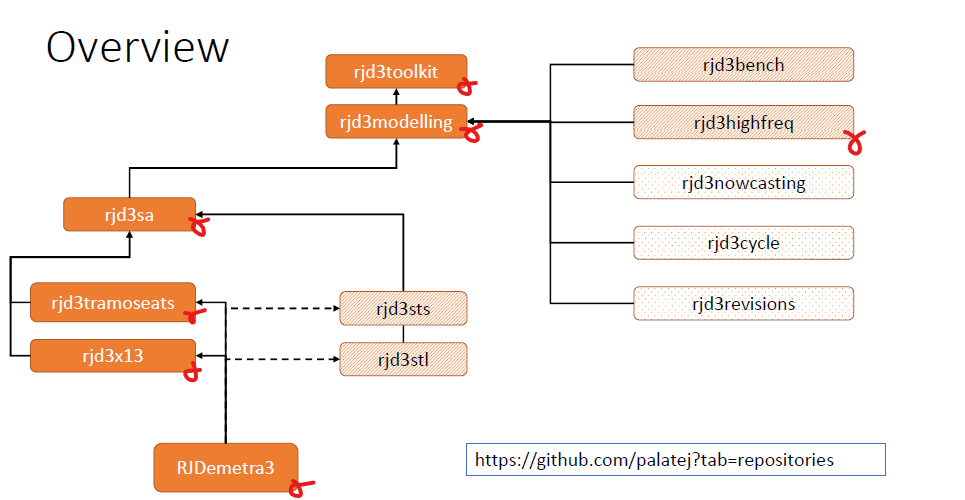
\includegraphics{img/Schema_JP_orga_packages.png}
\end{frame}

\begin{frame}{Seasonal adjustment algorithms in JDemetra+ version 3}
\protect\hypertarget{seasonal-adjustment-algorithms-in-jdemetra-version-3}{}
For seasonal adjustment, specifically, JDemetra+ contains:

\begin{itemize}
\tightlist
\item
  X13-Arima (GUI and R)
\item
  Tramo-Seats (GUI and R)
\item
  STL (R only)
\item
  Structural Time Series (SSF framework) (R only)
\end{itemize}

All of these algorithms can be used with HF data.

For X13-Arima and Tramo-Seats some illustrations are available only in
GUI. (auxiliary tools like: spectral analysis, sliding spans, revision
history\ldots)

Scope of this webinar: SA with X-13 and Tramo-Seats, including HF data
\end{frame}

\hypertarget{setting-up-your-work-environment}{%
\section{Setting up your work
environment}\label{setting-up-your-work-environment}}

\begin{frame}[fragile]{Installing packages (1/2)}
\protect\hypertarget{installing-packages-12}{}
Version 2: RJDemetra is on CRAN

\begin{Shaded}
\begin{Highlighting}[]
\FunctionTok{install.packages}\NormalTok{(}\StringTok{"RJDemetra"}\NormalTok{)}
\FunctionTok{library}\NormalTok{(}\StringTok{"RJDemetra"}\NormalTok{)}
\end{Highlighting}
\end{Shaded}

In part 3 and 4 we will also use

\begin{itemize}
\item
  JDCruncheR (based on cruncher output) To install it: download the
  \textbf{.zip} or \textbf{.tar.gz} file from
  \url{https://github.com/InseeFr/JDCruncheR/releases}.
\item
  rjdworkspace (based on RJDemetra) To install it: download the
  \textbf{.zip} or \textbf{.tar.gz} file from
  \url{https://github.com/InseeFrLab/rjdworkspace/releases}.
\end{itemize}

You can run v2 and v3 simultaneously

Version 3 requires Java \faIcon{java} \(\geq\) 17 (see
\url{https://github.com/jdemetra/rjdemetra/wiki/Installation-manual})
\end{frame}

\begin{frame}[fragile]{Installing packages (2/2)}
\protect\hypertarget{installing-packages-22}{}
Installing latest version from GitHub (as not on CRAN yet)

\begin{Shaded}
\begin{Highlighting}[]
\CommentTok{\# install.packages("remotes")}

\NormalTok{remotes}\SpecialCharTok{::}\FunctionTok{install\_github}\NormalTok{(}\StringTok{"palatej/rjdemetra3"}\NormalTok{)}

\NormalTok{remotes}\SpecialCharTok{::}\FunctionTok{install\_github}\NormalTok{(}\StringTok{"palatej/rjd3toolkit"}\NormalTok{, }\AttributeTok{ref =} \StringTok{"v0.6.0"}\NormalTok{)}

\NormalTok{remotes}\SpecialCharTok{::}\FunctionTok{install\_github}\NormalTok{(}\StringTok{"palatej/rjd3modelling"}\NormalTok{, }\AttributeTok{ref =} \StringTok{"v0.6.0"}\NormalTok{)}
\NormalTok{remotes}\SpecialCharTok{::}\FunctionTok{install\_github}\NormalTok{(}\StringTok{"palatej/rjd3arima"}\NormalTok{, }\AttributeTok{ref =} \StringTok{"v0.6.0"}\NormalTok{)}
\NormalTok{remotes}\SpecialCharTok{::}\FunctionTok{install\_github}\NormalTok{(}\StringTok{"palatej/rjd3sa"}\NormalTok{, }\AttributeTok{ref =} \StringTok{"v0.6.0"}\NormalTok{)}

\NormalTok{remotes}\SpecialCharTok{::}\FunctionTok{install\_github}\NormalTok{(}\StringTok{"palatej/rjd3tramoseats"}\NormalTok{, }\AttributeTok{ref =} \StringTok{"v0.6.0"}\NormalTok{)}
\NormalTok{remotes}\SpecialCharTok{::}\FunctionTok{install\_github}\NormalTok{(}\StringTok{"palatej/rjd3x13"}\NormalTok{, }\AttributeTok{ref =} \StringTok{"v0.6.0"}\NormalTok{)}
\NormalTok{remotes}\SpecialCharTok{::}\FunctionTok{install\_github}\NormalTok{(}\StringTok{"palatej/rjdemetra3"}\NormalTok{, }\AttributeTok{ref =} \StringTok{"v0.6.0"}\NormalTok{)}

\NormalTok{remotes}\SpecialCharTok{::}\FunctionTok{install\_github}\NormalTok{(}\StringTok{"palatej/rjd3sts"}\NormalTok{, }\AttributeTok{ref =} \StringTok{"v0.5.0"}\NormalTok{)}
\NormalTok{remotes}\SpecialCharTok{::}\FunctionTok{install\_github}\NormalTok{(}\StringTok{"palatej/rjd3highfreq"}\NormalTok{, }\AttributeTok{ref =} \StringTok{"v0.5.0"}\NormalTok{)}
\NormalTok{remotes}\SpecialCharTok{::}\FunctionTok{install\_github}\NormalTok{(}\StringTok{"palatej/rjd3stl"}\NormalTok{, }\AttributeTok{ref =} \StringTok{"v0.5.0"}\NormalTok{)}
\NormalTok{remotes}\SpecialCharTok{::}\FunctionTok{install\_github}\NormalTok{(}\StringTok{"palatej/rjd3bench"}\NormalTok{, }\AttributeTok{ref =} \StringTok{"v0.5.0"}\NormalTok{)}
\CommentTok{\# options : INSTALL\_opts = "{-}{-}no{-}multiarch"}

\NormalTok{remotes}\SpecialCharTok{::}\FunctionTok{install\_github}\NormalTok{(}\StringTok{"AQLT/ggdemetra3"}\NormalTok{) }\CommentTok{\#additional graphics }
\end{Highlighting}
\end{Shaded}
\end{frame}

\end{document}
